\documentclass[11pt,a4paper]{article}

% ---------------------------------------------------------------- packages
\usepackage[T1]{fontenc}
\usepackage[utf8]{inputenc}
\usepackage{lmodern}
\usepackage{microtype}
\usepackage[a4paper,margin=2.5cm,headheight=14pt]{geometry}
\usepackage{amsmath,amssymb,amsthm,bm}
\usepackage{graphicx}
\usepackage{booktabs}
\usepackage{array}
\usepackage{enumitem}
\usepackage[dvipsnames]{xcolor}
\usepackage{titlesec}
\usepackage{fancyhdr}
\usepackage[most]{tcolorbox}
\usepackage{caption}
\usepackage[section]{placeins}
\usepackage[colorlinks=true,linkcolor=tealhead,urlcolor=tealhead,citecolor=tealhead]{hyperref}
\hypersetup{pdftitle={Label-Efficient Learning with Unsupervised Methods},
  pdfauthor={Xaysomvang (Tom) Thammavong},
  pdfsubject={Clustering, semi-supervised learning and anomaly detection - technical report},
  pdfkeywords={K-Means, Gaussian mixture, EM, BIC, semi-supervised learning, anomaly detection, MLOps}}

% ---------------------------------------------------------------- colours
\definecolor{tealhead}{HTML}{0F7567}
\definecolor{navy}{HTML}{1A3A6B}
\definecolor{lightblue}{HTML}{EEF3FB}
\definecolor{lightteal}{HTML}{E8F5F2}
\pagecolor{white}

% ---------------------------------------------------------------- headings
\titleformat{\section}{\Large\bfseries\color{tealhead}}{\thesection}{0.8em}{}[{\color{tealhead}\titlerule[0.8pt]}]
\titleformat{\subsection}{\large\bfseries\color{tealhead}}{\thesubsection}{0.7em}{}[{\color{tealhead}\titlerule[0.4pt]}]
\titleformat{\subsubsection}{\normalsize\bfseries\color{tealhead}}{\thesubsubsection}{0.6em}{}
\titlespacing*{\section}{0pt}{1.6em}{0.9em}
\titlespacing*{\subsection}{0pt}{1.2em}{0.7em}

% ---------------------------------------------------------------- header / footer
\pagestyle{fancy}
\fancyhf{}
\fancyhead[L]{\small\color{tealhead}Label-efficient learning with unsupervised methods}
\fancyhead[R]{\small\color{tealhead}\leftmark}
\fancyfoot[C]{\thepage}
\renewcommand{\headrulewidth}{0.4pt}
\renewcommand{\headrule}{\hbox to\headwidth{\color{tealhead}\leaders\hrule height \headrulewidth\hfill}}
\renewcommand{\sectionmark}[1]{\markboth{#1}{}}
\fancypagestyle{plain}{\fancyhf{}\fancyfoot[C]{\thepage}\renewcommand{\headrulewidth}{0pt}}

% ---------------------------------------------------------------- boxes
\newtcolorbox{proofbox}[1][]{enhanced, breakable, colback=lightblue, colframe=navy, coltitle=white,
  fonttitle=\bfseries, title={#1}, boxrule=0.6pt, arc=2pt, left=8pt, right=8pt, top=6pt, bottom=6pt}
\newtcolorbox{summarybox}[1][Summary]{enhanced, breakable, colback=lightteal, colframe=tealhead, coltitle=white,
  fonttitle=\bfseries, title={#1}, boxrule=0.6pt, arc=2pt, left=8pt, right=8pt, top=6pt, bottom=6pt}

% ---------------------------------------------------------------- notation
\newcommand{\R}{\mathbb{R}}
\newcommand{\E}{\mathbb{E}}
\newcommand{\x}{\mathbf{x}}
\newcommand{\z}{\mathbf{z}}
\newcommand{\vmu}{\boldsymbol{\mu}}
\newcommand{\vSigma}{\boldsymbol{\Sigma}}
\newcommand{\vtheta}{\boldsymbol{\theta}}
\newcommand{\N}{\mathcal{N}}
\DeclareMathOperator*{\argmin}{arg\,min}
\DeclareMathOperator*{\argmax}{arg\,max}
\DeclareMathOperator{\tr}{tr}

\captionsetup{font=small,labelfont={bf,color=tealhead}}
\setlist{itemsep=2pt,topsep=4pt}

\begin{document}

% ================================================================ title
\begin{center}
  {\color{tealhead}\rule{\linewidth}{1pt}}\\[0.6em]
  {\LARGE\bfseries Label-Efficient Learning with Unsupervised Methods}\\[0.4em]
  {\large Clustering, Semi-Supervised Learning and Anomaly Detection,\\ served as an end-to-end MLOps system}\\[0.8em]
  {\normalsize Xaysomvang (Tom) Thammavong \quad$\cdot$\quad Technical report, October 2026}\\[0.2em]
  {\small Code: \url{https://github.com/ToMooGo/unsupervised-learning-mlops}}\\[0.4em]
  {\color{tealhead}\rule{\linewidth}{1pt}}
\end{center}

\noindent
Labelled data is expensive; unlabelled data is cheap. This report develops three ways of using unsupervised
learning to get more out of fewer labels, following the methods of Géron, \emph{Hands-On Machine Learning}
(2nd ed., Chapters~8 and~9), and derives the mathematics behind each step. Part~A uses K-Means distances as
features for a classifier; Part~B labels only cluster-representative images and propagates their labels; Part~C
detects anomalous inputs with a Gaussian mixture density. The final section describes how the three models are
trained, gated, deployed and monitored. The numbers quoted here are produced by the pipeline
(\texttt{reports/metrics.json}) or by the executed notebooks in the repository.

\tableofcontents
\clearpage

% ================================================================ 1
\section{Data and evaluation protocol}

\paragraph{Digits.} The scikit-learn digits dataset contains $1{,}797$ grey-scale images of $8\times 8$ pixels,
each pixel an integer in $\{0,\dots,16\}$. We write an image as a vector $\x\in\R^{n}$ with $n=64$ and its label
as $y\in\{0,\dots,9\}$. A random 75/25 split (seed 42) gives $m=1{,}347$ training and $450$ test images, as in the
book.

\paragraph{Why several splits.} With $450$ test images one misclassification moves accuracy by
\begin{equation}
  \frac{1}{450} = 0.22\ \text{percentage points (pp)},
\end{equation}
so a single split cannot distinguish models that differ by a few tenths of a point. We therefore repeat the key
comparisons on five further random splits (seeds $0,\dots,4$), re-tuning every hyperparameter inside each split on
its training set only, and report the mean $\pm$ standard deviation.

\paragraph{Anomaly benchmarks with ground truth.} The book's anomaly-detection examples have no labelled
anomalies. We generate the book's two synthetic datasets (three Gaussian blobs with weights $0.4,0.4,0.2$, and the
two moons) and inject a known contamination $q=4\%$ of uniformly scattered outliers. Outliers are rejection-sampled
so that they are genuinely anomalous: at least $3$ Mahalanobis units from every blob, or at least $0.15$ from every
moon point. With $1{,}000$ inliers this gives
\begin{equation}
  n_{\text{out}} = \operatorname{round}\!\left(1000\cdot\frac{q}{1-q}\right)
  = \operatorname{round}\!\left(\frac{40}{0.96}\right) = 42
\end{equation}
outliers per dataset, i.e.\ a contamination of $42/1042 = 4.03\%$.

\paragraph{Metrics.} For a detector that flags a set $F$ of points, with $P$ the set of true outliers,
\begin{align}
  \text{precision} &= \frac{|F\cap P|}{|F|}, &
  \text{recall} &= \frac{|F\cap P|}{|P|}, &
  F_1 &= \frac{2\,\text{precision}\cdot\text{recall}}{\text{precision}+\text{recall}}.
\end{align}
ROC-AUC is computed from a continuous anomaly score and does not depend on the threshold.

% ================================================================ 2
\section{Part A: K-Means as a feature-engineering step}

\subsection{The K-Means objective and Lloyd's algorithm}
K-Means partitions the training set into $k$ clusters with centroids $\vmu_1,\dots,\vmu_k$ by minimising the
\emph{inertia} (within-cluster sum of squares)
\begin{equation}\label{eq:inertia}
  J(c,\vmu) = \sum_{i=1}^{m} \bigl\lVert \x_i - \vmu_{c(i)} \bigr\rVert^2,
\end{equation}
where $c(i)\in\{1,\dots,k\}$ is the cluster of $\x_i$. Lloyd's algorithm alternates two steps:
\begin{align}
  \text{assignment:}\quad & c(i) \leftarrow \argmin_{j}\ \lVert \x_i - \vmu_j \rVert^2, \label{eq:assign}\\
  \text{update:}\quad & \vmu_j \leftarrow \frac{1}{|C_j|}\sum_{i\in C_j}\x_i,\qquad C_j=\{i : c(i)=j\}. \label{eq:update}
\end{align}

\begin{proofbox}[Proposition 1. The centroid update minimises the inertia of a fixed cluster]
For a fixed assignment, the contribution of cluster $j$ to $J$ is
$J_j(\vmu_j)=\sum_{i\in C_j}\lVert\x_i-\vmu_j\rVert^2$. Expanding the squared norm,
\begin{equation*}
  J_j(\vmu_j)=\sum_{i\in C_j}\left(\x_i^\top\x_i-2\,\x_i^\top\vmu_j+\vmu_j^\top\vmu_j\right).
\end{equation*}
Differentiating with respect to $\vmu_j$ term by term,
\begin{equation*}
  \nabla_{\vmu_j}J_j=\sum_{i\in C_j}\left(-2\,\x_i+2\,\vmu_j\right)=-2\sum_{i\in C_j}\x_i+2\,|C_j|\,\vmu_j .
\end{equation*}
Setting the gradient to zero gives $\vmu_j=\frac{1}{|C_j|}\sum_{i\in C_j}\x_i$, which is \eqref{eq:update}.
The Hessian is $\nabla^2_{\vmu_j}J_j=2|C_j|\,I\succ 0$, so $J_j$ is strictly convex and this stationary point is the
unique minimiser. \hfill$\square$
\end{proofbox}

\begin{proofbox}[Proposition 2. Lloyd's algorithm terminates]
The assignment step \eqref{eq:assign} chooses, for each $i$ separately, the centroid that minimises its own term
of \eqref{eq:inertia}, so it cannot increase $J$. By Proposition~1 the update step minimises each $J_j$ for the
current assignment, so it cannot increase $J$ either. Hence $J$ is non-increasing along the iterations. There are
at most $k^m$ assignments, and each is visited at most once while $J$ strictly decreases (ties broken
consistently). Therefore the algorithm reaches a fixed point after finitely many iterations. The fixed point is a
local minimum in general, which is why scikit-learn restarts from \texttt{n\_init}$=10$ random initialisations and
keeps the solution with the lowest $J$. \hfill$\square$
\end{proofbox}

\subsection{From clusters to features}
After fitting, every image is mapped to its vector of distances to the $k$ centroids,
\begin{equation}\label{eq:featuremap}
  \phi(\x) = \bigl(\lVert\x-\vmu_1\rVert,\ \lVert\x-\vmu_2\rVert,\ \dots,\ \lVert\x-\vmu_k\rVert\bigr)^\top\in\R^{k}.
\end{equation}
This is a non-linear map: a linear model in $\phi(\x)$ can carve out regions around each centroid, which a linear
model on raw pixels cannot. The features are then standardised component-wise,
\begin{equation}
  z_\ell = \frac{\phi_\ell(\x)-\bar\phi_\ell}{s_\ell},\qquad \ell=1,\dots,k,
\end{equation}
with $\bar\phi_\ell$ and $s_\ell$ the training mean and standard deviation (Section~\ref{sec:scaling} explains why).

\subsection{Multinomial logistic regression on the distance features}
For classes $c=0,\dots,9$ with parameter vectors $\vtheta_c$ (bias absorbed into $\z$), the model is the softmax
\begin{equation}
  p_c(\z)=\frac{\exp(\vtheta_c^\top\z)}{\sum_{c'}\exp(\vtheta_{c'}^\top\z)} .
\end{equation}
With one-hot targets $y_{ic}$, the regularised cross-entropy minimised by \texttt{lbfgs} is
\begin{equation}\label{eq:ce}
  L(\vtheta)= -\sum_{i=1}^{m}\sum_{c}y_{ic}\log p_c(\z_i)+\frac{1}{2C}\sum_c\lVert\vtheta_c\rVert^2 .
\end{equation}

\begin{proofbox}[Proposition 3. Gradient of the cross-entropy]
Write $a_{ic}=\vtheta_c^\top\z_i$ and $\log p_c(\z_i)=a_{ic}-\log\sum_{c'}e^{a_{ic'}}$. For a fixed class $d$,
\begin{equation*}
  \frac{\partial \log p_c(\z_i)}{\partial a_{id}}
  =\delta_{cd}-\frac{e^{a_{id}}}{\sum_{c'}e^{a_{ic'}}}=\delta_{cd}-p_d(\z_i).
\end{equation*}
Using $\sum_c y_{ic}=1$,
\begin{equation*}
  \frac{\partial}{\partial a_{id}}\Bigl(-\sum_c y_{ic}\log p_c(\z_i)\Bigr)
  =-\sum_c y_{ic}\bigl(\delta_{cd}-p_d(\z_i)\bigr)=p_d(\z_i)-y_{id}.
\end{equation*}
Since $\partial a_{id}/\partial\vtheta_d=\z_i$, the chain rule gives
\begin{equation*}
  \nabla_{\vtheta_d}L=\sum_{i=1}^{m}\bigl(p_d(\z_i)-y_{id}\bigr)\z_i+\frac{1}{C}\vtheta_d .
\end{equation*}
\hfill$\square$
\end{proofbox}

\subsection{Why the distance features must be scaled}\label{sec:scaling}
The gradient in Proposition~3 is a weighted sum of the feature vectors $\z_i$, so the curvature of $L$ is governed
by the Gram matrix $Z^\top Z$ of the features (with a column of ones for the bias). Raw distances are all positive
and large compared with their spread: for $k=50$ the median distance is $45$, most values lie between $29$ and
$56$, and the average per-feature standard deviation is only $7.7$. The common offset creates one direction of very
large curvature next to many directions of small curvature. The condition number of $Z^\top Z$ is
$2.2\times10^{8}$ on raw distances and $4.7\times10^{3}$ after standardisation, a reduction of more than four orders
of magnitude. A quasi-Newton method converges much more slowly on an ill-conditioned problem. On our split with
$k=50$, \texttt{lbfgs} converged in $44$ iterations on scaled features versus $1{,}268$ on raw distances, and during
the full grid search some raw-distance fits stopped at the $10{,}000$-iteration limit.
With an identical grid ($k=10,15,\dots,95$), the scaled variant reached a
cross-validated accuracy of $95.9\%$ against $95.6\%$, with the same test accuracy ($97.6\%$), and fitted the grid
$6.3$ times faster ($7$\,s versus $46$\,s).

\subsection{Choosing $k$ and results}
Because K-Means is only a preprocessing step, the right $k$ is the one that maximises the \emph{classifier's}
cross-validated accuracy, not the one that minimises inertia or maximises the silhouette score. A 3-fold
\texttt{GridSearchCV} over $k=2,\dots,99$ on the training set selects $k=81$ (CV accuracy $96.0\%$).
Figure~\ref{fig:ksel} shows the unsupervised criteria preferring far smaller $k$.

\begin{figure}[h]
  \centering
  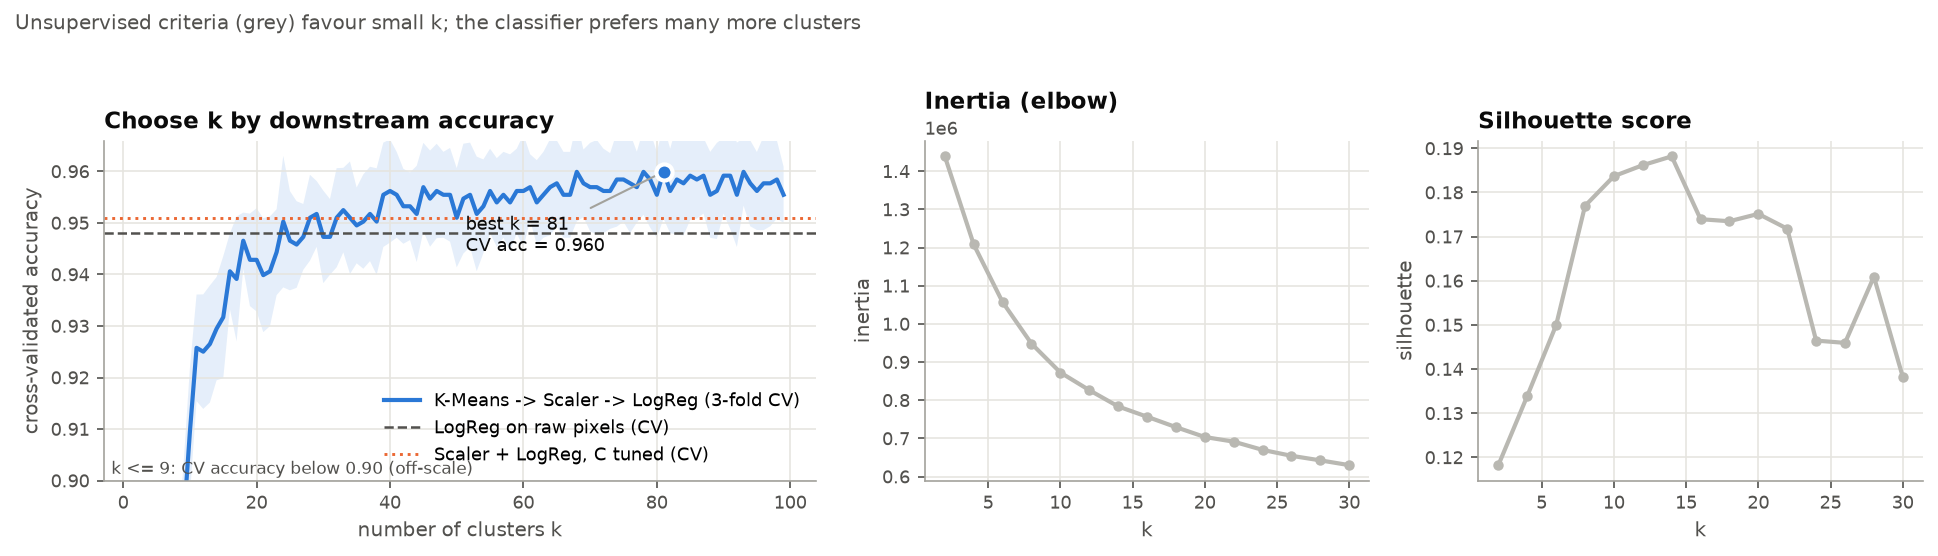
\includegraphics[width=\linewidth]{../figures/a_k_selection.png}
  \caption{Left: CV accuracy of the K-Means $\to$ Logistic Regression pipeline versus $k$ ($\pm1$ std band);
  dashed line: Logistic Regression on raw pixels. Middle and right: inertia and silhouette score.}
  \label{fig:ksel}
\end{figure}

\paragraph{A fair comparison.} The book compares against Logistic Regression on raw pixels with default
settings, while the pipeline also benefits from scaling and from a $98$-value search over $k$. We therefore add a
strong baseline: StandardScaler followed by Logistic Regression with the regularisation strength $C$ tuned by the
same 3-fold cross-validation over $C\in\{0.01,0.03,\dots,100\}$. On the five extra splits, every hyperparameter
($k$ on the coarse grid $10,20,\dots,90$, and $C$) is re-tuned on each split's training set.

\begin{table}[h]
  \centering
  \begin{tabular}{lcc}
    \toprule
    Model & Split 42 & Mean $\pm$ std over 5 splits \\
    \midrule
    Logistic Regression, raw pixels (book) & $97.3\%$ & $95.6\% \pm 1.0\%$ \\
    StandardScaler $\to$ LogReg ($C$ tuned) & $97.1\%$ & $96.3\% \pm 1.2\%$ \\
    K-Means $\to$ StandardScaler $\to$ LogReg ($k$ tuned) & $\mathbf{97.6\%}$ & $\mathbf{96.9\% \pm 0.9\%}$ \\
    \bottomrule
  \end{tabular}
  \caption{Part A test accuracy. On split 42 the difference between the book baseline and the pipeline is
  $12\to11$ errors. Over five splits the pipeline beats the book baseline on $5/5$ splits ($+1.29$\,pp) and the
  strong baseline on $4/5$ ($+0.62$\,pp).}
\end{table}

\begin{summarybox}[Summary: Part A]
\begin{itemize}[leftmargin=1.2em]
  \item Distances to K-Means centroids are a useful non-linear feature map for a linear classifier. The gain is
        $+0.6$\,pp over a tuned, scaled baseline (better on $4/5$ splits) and $+1.3$\,pp over the book's baseline.
        It is real but modest, and close to the resolution of a 450-image test set.
  \item $k$ is a classifier hyperparameter and is chosen by cross-validated accuracy ($k=81$), not by inertia.
  \item Standardising the distances fixes the conditioning of the optimisation: $44$ instead of $1{,}268$
        iterations, a $6\times$ faster grid search, and equal accuracy.
\end{itemize}
\end{summarybox}

% ================================================================ 3
\section{Part B: Semi-supervised learning with 50 labels}

\subsection{Representative images}
Suppose only $k=50$ images can be labelled ($3.7\%$ of the training set). Cluster the training set into $k$
clusters and, for each centroid, pick the image closest to it:
\begin{equation}
  r_j=\argmin_{i\in\{1,\dots,m\}}\ \lVert\x_i-\vmu_j\rVert,\qquad j=1,\dots,k.
\end{equation}
These \emph{representative} images cover the modes of the data, whereas 50 random images over-sample common
writing styles and miss rare ones. A human (or, in reproducible runs, the ground truth acting as an oracle) labels
$y_{r_1},\dots,y_{r_k}$.

\subsection{Label propagation}
\emph{Full propagation} gives every image the label of its cluster's representative,
\begin{equation}
  \hat y_i=y_{r_{c(i)}} .
\end{equation}
Images near a cluster boundary are often a different digit, so we keep only the images closest to their centroid.
With $d_i=\lVert\x_i-\vmu_{c(i)}\rVert$ and $Q_j(p)$ the $p$-th percentile of $\{d_i : i\in C_j\}$, the
\emph{partially propagated} training set is
\begin{equation}
  S_p=\bigcup_{j=1}^{k}\{\,i\in C_j : d_i\le Q_j(p)\,\}\ \cup\ \{r_1,\dots,r_k\}.
\end{equation}
Smaller $p$ means fewer but more reliable pseudo-labels. On our split, $p=20$ keeps $288$ images whose
propagated labels are $98.3\%$ correct, against $93.5\%$ for full propagation (Figure~\ref{fig:semi}).

\subsection{How much does one wrong label cost?}
Let $n_j=|C_j|$. With partial propagation, cluster $j$ contributes about $p\,n_j/100$ images to $S_p$, so
\begin{equation}
  |S_p|\approx\frac{p}{100}\sum_{j=1}^{k}n_j=\frac{p\,m}{100}.
\end{equation}
If the representative label of cluster $j$ is wrong, every one of its propagated images is wrong, which is a share
\begin{equation}
  \frac{p\,n_j/100}{p\,m/100}=\frac{n_j}{m}\approx\frac{1}{k}=\frac{1}{50}=2\%
\end{equation}
of the training set. These mislabelled images all lie in one region of input space, so the model learns a wrong
decision there rather than averaging out the noise. Empirically, one random wrong representative label lowers
test accuracy by $2.4$\,pp on average ($92.4\%\to90.1\%$, worst case $88.4\%$), two by $5.3$\,pp, and five by
$12.5$\,pp. In ordinary supervised learning one wrong label out of $1{,}347$ would be invisible. This
sensitivity is the reason the deployment pipeline has a champion-versus-challenger gate (Section~\ref{sec:system}).

\subsection{Active learning by uncertainty sampling}
To spend further labels well, the model asks about the unlabelled images it is least sure of:
\begin{equation}
  i^\star=\argmin_{i\notin S}\ \max_{c}\ p_c(\x_i).
\end{equation}
Adding $10$ such labels per round for $5$ rounds ($50\to100$ human labels) raises test accuracy from $92.4\%$ to
$93.8\%$.

\begin{figure}[h]
  \centering
  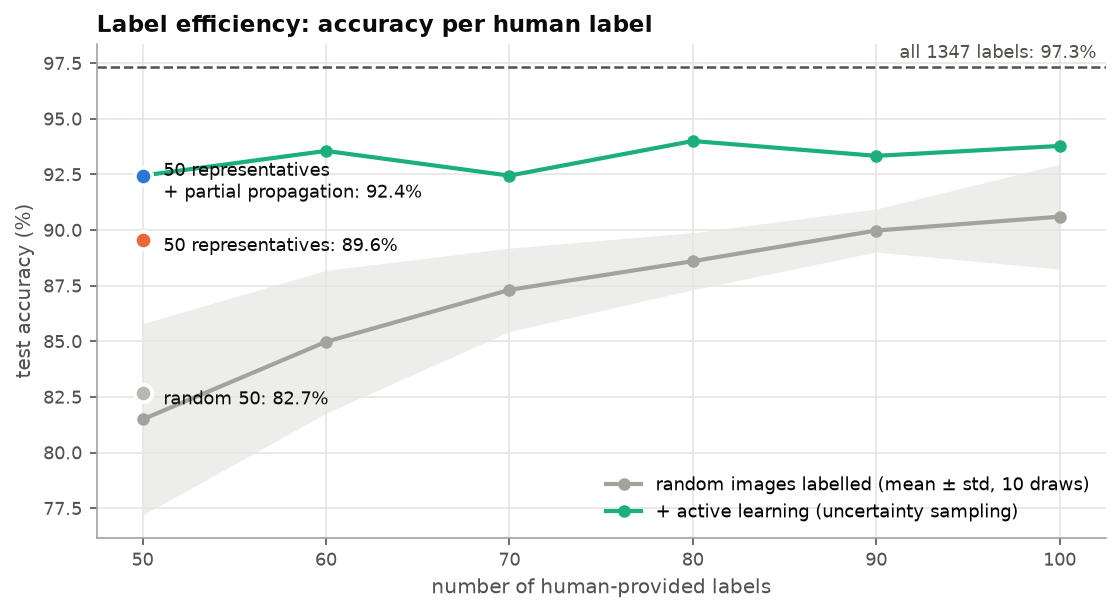
\includegraphics[width=0.78\linewidth]{../figures/b_label_efficiency.png}
  \caption{Test accuracy versus number of human labels. Grey: random images (mean $\pm$ std over 10 draws).
  Dots at 50 labels: random, representatives, representatives with partial propagation. Aqua: active learning.}
  \label{fig:semi}
\end{figure}

\begin{table}[h]
  \centering
  \begin{tabular}{lccc}
    \toprule
    Training labels & Images & Label accuracy & Test accuracy\\
    \midrule
    50 random images & 50 & $100\%$ & $82.7\%$\\
    50 representatives & 50 & $100\%$ & $89.6\%$\\
    \quad + full propagation & 1{,}347 & $93.5\%$ & $90.9\%$\\
    \quad + partial propagation ($p=20$) & 288 & $98.3\%$ & $\mathbf{92.4\%}$\\
    All true labels (upper bound) & 1{,}347 & $100\%$ & $97.3\%$\\
    \bottomrule
  \end{tabular}
  \caption{Part B on split 42. Over five further splits: random 50 labels $83.4\%\pm2.5\%$ versus partial
  propagation $92.4\%\pm1.0\%$, with propagated-label accuracy $98.9\%$.}
\end{table}

\begin{summarybox}[Summary: Part B]
\begin{itemize}[leftmargin=1.2em]
  \item Choosing \emph{which} 50 images to label matters: representatives plus partial propagation reach
        $92.4\%$ against $82.7\%$ for random labels, using $3.7\%$ of the labels.
  \item Partial propagation trades coverage for label quality ($98.3\%$ correct pseudo-labels).
  \item Each representative label stands for about $1/k$ of the training data, so labelling mistakes are
        amplified. Label quality must be checked before deployment.
\end{itemize}
\end{summarybox}

% ================================================================ 4
\section{Part C: Anomaly detection with Gaussian mixtures}

\subsection{The model}
A Gaussian mixture model (GMM) assumes each instance is generated by first drawing a cluster
$z\sim\text{Categorical}(\phi_1,\dots,\phi_k)$ and then $\x\mid z=j\sim\N(\vmu_j,\vSigma_j)$. Marginalising over
$z$ gives the density
\begin{equation}\label{eq:gmm}
  p(\x)=\sum_{j=1}^{k}\phi_j\,\N(\x;\vmu_j,\vSigma_j),\qquad
  \N(\x;\vmu,\vSigma)=\frac{\exp\!\bigl(-\tfrac12(\x-\vmu)^\top\vSigma^{-1}(\x-\vmu)\bigr)}{(2\pi)^{n/2}|\vSigma|^{1/2}},
\end{equation}
with $\phi_j\ge0$ and $\sum_j\phi_j=1$. The log-likelihood of the training set is
\begin{equation}\label{eq:loglik}
  \ell(\vtheta)=\sum_{i=1}^{m}\log\sum_{j=1}^{k}\phi_j\,\N(\x_i;\vmu_j,\vSigma_j).
\end{equation}
The logarithm of a sum has no closed-form maximiser, which motivates the Expectation-Maximisation (EM)
algorithm.

\subsection{Expectation-Maximisation}
\paragraph{E-step.} With the current parameters, Bayes' theorem gives the \emph{responsibility} of cluster $j$ for
instance $i$:
\begin{equation}\label{eq:resp}
  \gamma_{ij}=P(z_i=j\mid\x_i)=\frac{\phi_j\,\N(\x_i;\vmu_j,\vSigma_j)}{\sum_{l=1}^{k}\phi_l\,\N(\x_i;\vmu_l,\vSigma_l)} .
\end{equation}
\paragraph{M-step.} Holding the $\gamma_{ij}$ fixed, maximise the expected complete-data log-likelihood
\begin{equation}\label{eq:Q}
  Q(\vtheta)=\sum_{i=1}^{m}\sum_{j=1}^{k}\gamma_{ij}\Bigl[\log\phi_j-\tfrac{n}{2}\log 2\pi-\tfrac12\log|\vSigma_j|
  -\tfrac12(\x_i-\vmu_j)^\top\vSigma_j^{-1}(\x_i-\vmu_j)\Bigr].
\end{equation}
Write $N_j=\sum_{i}\gamma_{ij}$ for the effective number of instances in cluster $j$.

\begin{proofbox}[Proposition 4. M-step update of the weights]
Only the term $\sum_{i,j}\gamma_{ij}\log\phi_j=\sum_j N_j\log\phi_j$ depends on $\phi$. We maximise it subject to
$\sum_j\phi_j=1$ with a Lagrange multiplier $\lambda$:
\begin{equation*}
  \mathcal{L}(\phi,\lambda)=\sum_{j=1}^{k}N_j\log\phi_j+\lambda\Bigl(1-\sum_{j=1}^{k}\phi_j\Bigr).
\end{equation*}
Setting $\partial\mathcal{L}/\partial\phi_j=N_j/\phi_j-\lambda=0$ gives $\phi_j=N_j/\lambda$. Summing over $j$ and
using the constraint, $1=\sum_j N_j/\lambda=m/\lambda$, since $\sum_j\gamma_{ij}=1$ for every $i$. Hence
$\lambda=m$ and
\begin{equation*}
  \phi_j=\frac{N_j}{m}.
\end{equation*}
\hfill$\square$
\end{proofbox}

\begin{proofbox}[Proposition 5. M-step update of the means]
The terms of \eqref{eq:Q} involving $\vmu_j$ are $-\tfrac12\sum_i\gamma_{ij}(\x_i-\vmu_j)^\top\vSigma_j^{-1}(\x_i-\vmu_j)$.
Since $\nabla_{\mathbf{a}}\,\mathbf{a}^\top A\,\mathbf{a}=2A\mathbf{a}$ for symmetric $A$, and
$\partial(\x_i-\vmu_j)/\partial\vmu_j=-I$,
\begin{equation*}
  \nabla_{\vmu_j}Q=\sum_{i=1}^{m}\gamma_{ij}\,\vSigma_j^{-1}(\x_i-\vmu_j)
  =\vSigma_j^{-1}\Bigl(\sum_{i}\gamma_{ij}\x_i-N_j\vmu_j\Bigr).
\end{equation*}
$\vSigma_j^{-1}$ is invertible, so setting the gradient to zero gives
\begin{equation*}
  \vmu_j=\frac{1}{N_j}\sum_{i=1}^{m}\gamma_{ij}\,\x_i ,
\end{equation*}
a responsibility-weighted average. With hard responsibilities ($\gamma_{ij}\in\{0,1\}$) this is exactly the
K-Means update \eqref{eq:update}. This is the sense in which EM generalises K-Means. \hfill$\square$
\end{proofbox}

\begin{proofbox}[Proposition 6. M-step update of the covariances]
Let $\Lambda_j=\vSigma_j^{-1}$ and use $\log|\vSigma_j|=-\log|\Lambda_j|$ and
$(\x-\vmu)^\top\Lambda(\x-\vmu)=\tr\!\bigl(\Lambda(\x-\vmu)(\x-\vmu)^\top\bigr)$. The $\Lambda_j$-dependent part
of \eqref{eq:Q} is
\begin{equation*}
  Q_j(\Lambda_j)=\tfrac12 N_j\log|\Lambda_j|-\tfrac12\tr\!\Bigl(\Lambda_j\sum_i\gamma_{ij}(\x_i-\vmu_j)(\x_i-\vmu_j)^\top\Bigr).
\end{equation*}
Using the matrix identities $\nabla_\Lambda\log|\Lambda|=\Lambda^{-1}$ and $\nabla_\Lambda\tr(\Lambda B)=B^\top$,
\begin{equation*}
  \nabla_{\Lambda_j}Q_j=\tfrac12N_j\Lambda_j^{-1}-\tfrac12\sum_i\gamma_{ij}(\x_i-\vmu_j)(\x_i-\vmu_j)^\top=0
  \;\Longrightarrow\;
  \vSigma_j=\frac{1}{N_j}\sum_{i=1}^{m}\gamma_{ij}(\x_i-\vmu_j)(\x_i-\vmu_j)^\top .
\end{equation*}
scikit-learn adds $\texttt{reg\_covar}\cdot I=10^{-6}I$ to keep $\vSigma_j$ positive definite. \hfill$\square$
\end{proofbox}

Each EM iteration cannot decrease $\ell(\vtheta)$, but, like K-Means, EM can converge to a poor local optimum.
It is therefore restarted from several initialisations (\texttt{n\_init}) and the best run is kept.

\subsection{Choosing $k$ and the covariance type: BIC and AIC}
Inertia and the silhouette score assume spherical, equally sized clusters, so for GMMs we use information
criteria. With $\hat L$ the maximised likelihood, $p$ the number of free parameters and $m$ the number of
instances,
\begin{align}
  \text{BIC}&=p\log m-2\log\hat L, \label{eq:bic}\\
  \text{AIC}&=2p-2\log\hat L .
\end{align}
Both reward fit and penalise complexity; BIC's penalty grows with $m$ and selects simpler models.

\begin{proofbox}[Parameter counts for $k$ components in $n$ dimensions]
There are $k-1$ free weights (they sum to one) and $kn$ mean coordinates. A symmetric $n\times n$ covariance has
$n(n+1)/2$ free entries. Therefore
\begin{align*}
  p_{\text{full}}&=(k-1)+kn+k\,\tfrac{n(n+1)}{2}, &
  p_{\text{tied}}&=(k-1)+kn+\tfrac{n(n+1)}{2},\\
  p_{\text{diag}}&=(k-1)+kn+kn, &
  p_{\text{spherical}}&=(k-1)+kn+k.
\end{align*}
For the digits detector selected below ($k=6$, full covariance, $n=28$ after PCA):
\begin{equation*}
  p=5+6\cdot28+6\cdot\tfrac{28\cdot29}{2}=5+168+2436=2609,
\end{equation*}
and the BIC penalty is $p\log m=2609\cdot\log(1347)=2609\cdot7.206\approx18{,}800$ nats.
\end{proofbox}

\subsection{Reducing the dimension with PCA}
In $64$ dimensions a single full covariance already has $64\cdot65/2=2080$ parameters, against $1{,}347$ training
images. Following the book's Chapter~8, we first project onto the $d$ leading principal components, choosing the
smallest $d$ that keeps $95\%$ of the variance:
\begin{equation}
  d=\min\Bigl\{d' : \frac{\sum_{i=1}^{d'}\lambda_i}{\sum_{i=1}^{n}\lambda_i}\ge0.95\Bigr\},
\end{equation}
where $\lambda_1\ge\lambda_2\ge\dots$ are the eigenvalues of the training covariance matrix. This gives $d=28$. BIC
over $k=1,\dots,15$ and the four covariance types then selects $k=6$ with full covariances.

\subsection{The density threshold and its calibration}
The anomaly score is the log-density $s(\x)=\log p(\x)$. Given the expected contamination $q=4\%$, the book sets
the threshold $\tau$ to the $q$-quantile of the training scores and flags $\x$ when $s(\x)<\tau$.

This threshold is optimistic. EM chooses $\vtheta$ to maximise the sum of the \emph{training} scores, so training
images have systematically higher density than unseen images from the same distribution. A threshold taken from
training scores therefore flags more than $q$ of new normal data. We measured $8.9\%$ instead of $4\%$ on the clean
test digits. The fix is to fit the GMM on $75\%$ of the training images and take $\tau$ from the held-out $25\%$.

\begin{proofbox}[Proposition 7. A held-out quantile controls the false-alarm rate]
Let $s_1,\dots,s_N$ be the scores of $N$ held-out normal images and $s_{N+1}$ the score of a new normal image.
Assume the fitted model is independent of these $N+1$ images and the scores are exchangeable with no ties. Then the
rank $R$ of $s_{N+1}$ among all $N+1$ scores is uniformly distributed on $\{1,\dots,N+1\}$. Let $\tau=s_{(\ell)}$
be the $\ell$-th smallest held-out score. The new image is flagged exactly when it ranks below $s_{(\ell)}$, so
\begin{equation*}
  P\bigl(s_{N+1}<s_{(\ell)}\bigr)=P(R\le\ell)=\frac{\ell}{N+1}.
\end{equation*}
Choosing $\ell\approx qN$ makes the expected false-alarm rate approximately $q$. Here $N=337$ and the empirical
4th percentile lies between the 14th and 15th smallest held-out scores ($\ell\approx14.4$), so the expected rate is
$14.4/338\approx4.3\%$. The observed $2.9\%$ (13 of 450 clean test images) is about $1.5$ binomial standard
deviations below this, where one standard deviation is $\sqrt{0.043\cdot0.957/450}\approx0.96$\,pp. Training scores do not satisfy the exchangeability assumption, because the
model was fitted to them. This is exactly why the training quantile fails. \hfill$\square$
\end{proofbox}

\subsection{DBSCAN with a label-free choice of $\varepsilon$}
DBSCAN marks an instance as a \emph{core} instance if at least \texttt{min\_samples}$=5$ instances lie within
distance $\varepsilon$. Clusters are chains of neighbouring core instances, and instances that are neither core
nor near one are \emph{noise}, which we treat as anomalies. The result is very sensitive to $\varepsilon$: on the
moons, $\varepsilon=0.05$ gives $7$ clusters and $11.4\%$ noise, while $\varepsilon=0.2$ gives the $2$ moons. To
compare DBSCAN fairly with the GMM, we give it the same prior and \emph{no labels}: we choose $\varepsilon$ on a
geometric grid so that the noise fraction is closest to $q$.

\paragraph{Why precision equals recall in the GMM rows.} With the threshold at the 4th percentile of the
$M=1042$ scores, the GMM flags $|F|=42$ points, which is exactly the number of injected outliers $|P|=42$. When
$|F|=|P|$,
\begin{equation}
  \text{precision}=\frac{|F\cap P|}{|F|}=\frac{|F\cap P|}{|P|}=\text{recall}=F_1 .
\end{equation}
DBSCAN's noise fraction only approximately equals $q$, so its precision and recall differ slightly.

\subsection{Results}
\begin{table}[h]
  \centering
  \begin{tabular}{lcc}
    \toprule
    $F_1$ (mean $\pm$ std over 5 random datasets) & Blobs (elliptical) & Moons (curved)\\
    \midrule
    GMM, $k$ and covariance type by BIC & $\mathbf{0.914\pm0.013}$ & $0.971\pm0.011$\\
    DBSCAN, label-free $\varepsilon$ & $0.884\pm0.024$ & $\mathbf{1.000\pm0.000}$\\
    Local Outlier Factor & $0.857\pm0.048$ & $1.000\pm0.000$\\
    Isolation Forest & $0.819\pm0.071$ & $0.810\pm0.053$\\
    Elliptic Envelope (Fast-MCD) & $0.667\pm0.081$ & $0.652\pm0.055$\\
    \bottomrule
  \end{tabular}
  \caption{Anomaly benchmark with $4\%$ injected outliers. The last three detectors are the book's other
  methods, included for reference. Fast-MCD assumes a single Gaussian and fails on multi-cluster data.}
\end{table}

\begin{figure}[h]
  \centering
  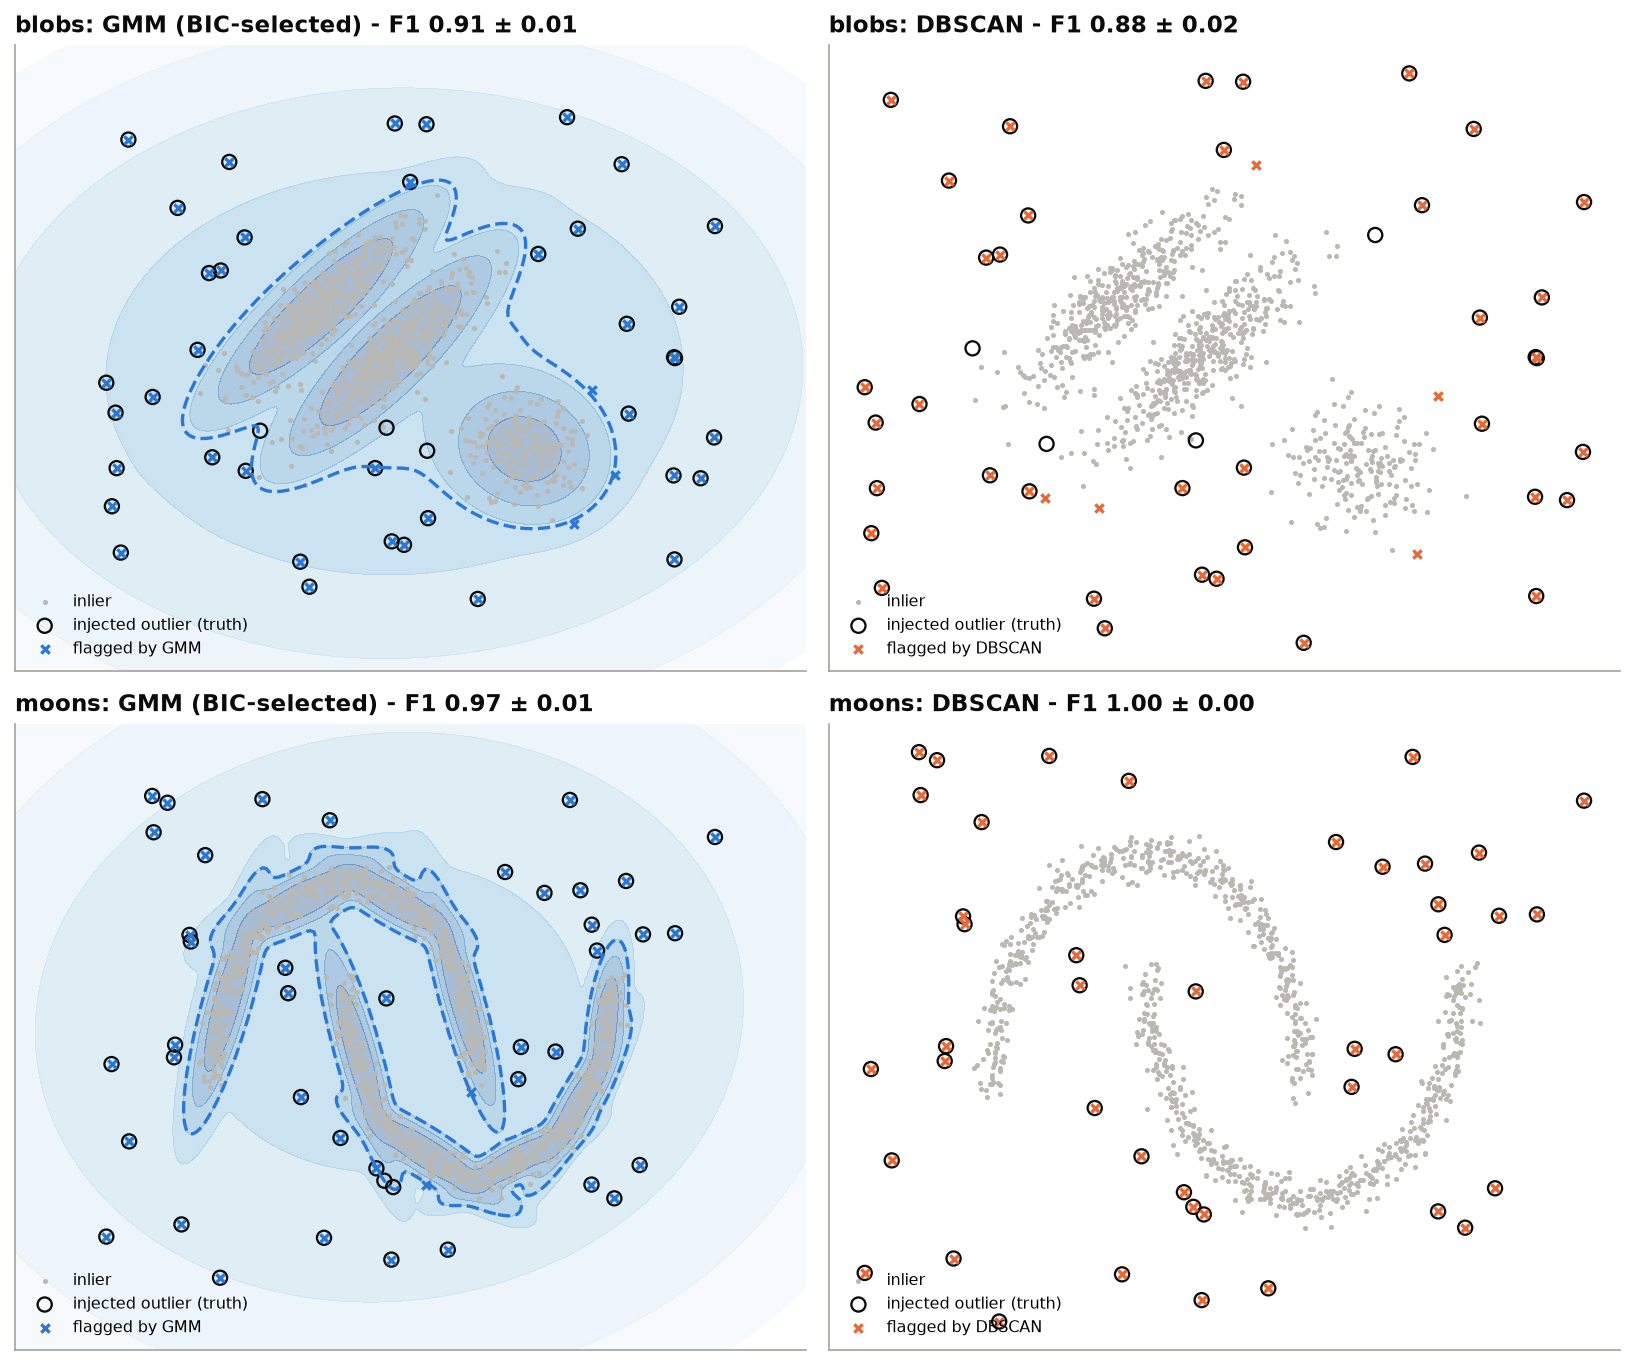
\includegraphics[width=0.92\linewidth]{../figures/c_synthetic_detection.png}
  \caption{GMM (left, with density contours and the threshold as a dashed line) and DBSCAN (right) on one blob
  dataset and one moon dataset. Circles mark the true outliers and crosses the flagged points.}
\end{figure}

\begin{figure}[h]
  \centering
  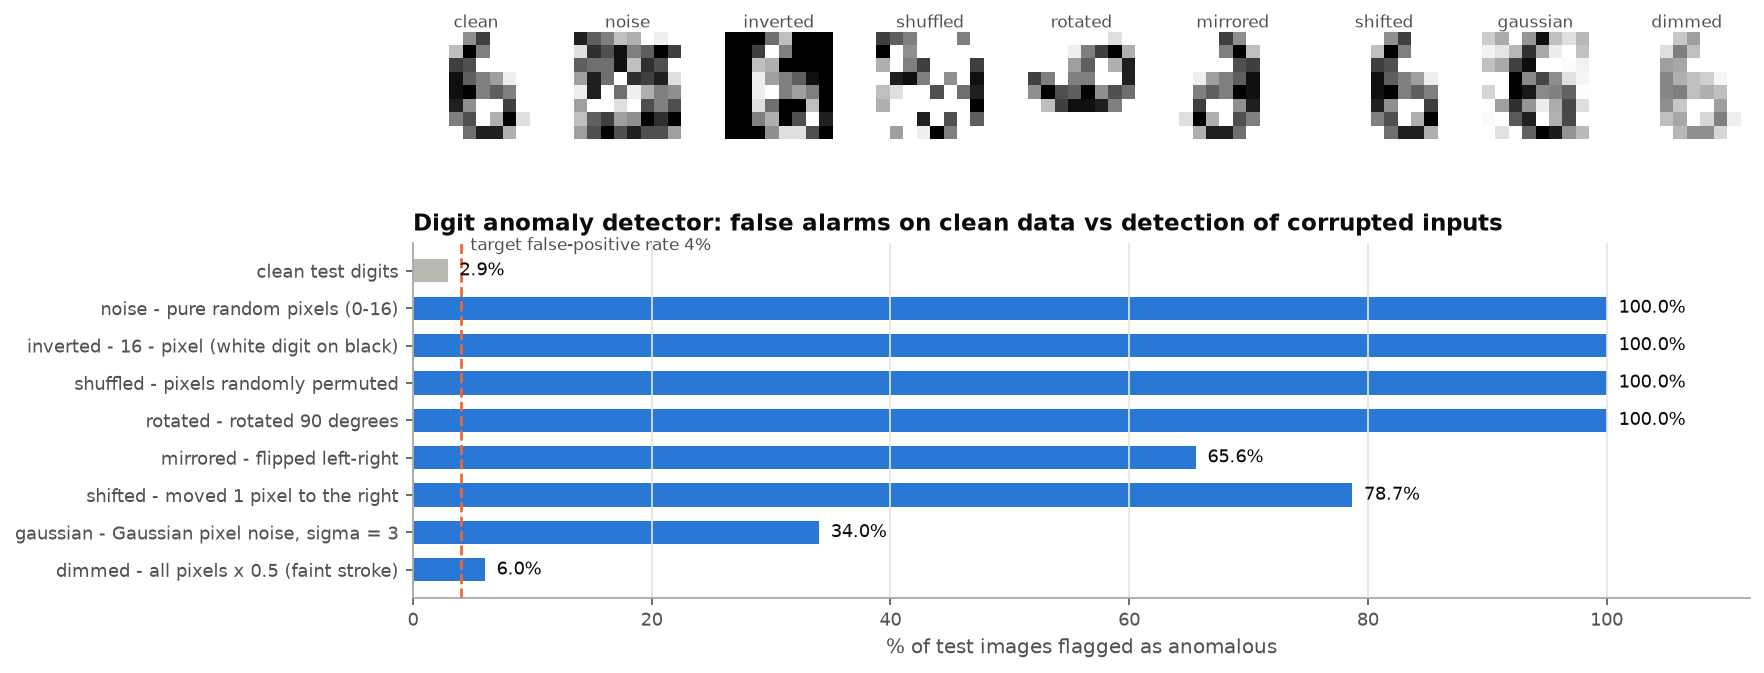
\includegraphics[width=\linewidth]{../figures/c_corruptions.png}
  \caption{Digit detector. False alarms on clean test digits ($2.9\%$) and detection rate for eight kinds of
  corrupted input. Structural corruptions are caught every time; dimmed digits and mild noise mostly are not.}
\end{figure}

On clean test digits, images that the detector flags are misclassified by the supervised model $30.8\%$ of the
time (4 of 13), against $1.6\%$ (7 of 437) for the rest. The detector is therefore a useful signal of when not to
trust a prediction. This matters because the classifier itself cannot abstain: softmax always outputs one of the
ten digits. On pure noise its average confidence is still $65\%$, and the detector flags all of these images.

\begin{summarybox}[Summary: Part C]
\begin{itemize}[leftmargin=1.2em]
  \item A GMM gives every input a calibrated ``have I seen data like this?'' score. EM generalises K-Means with
        soft assignments, and BIC/AIC choose the number and shape of the components.
  \item On elliptical clusters the GMM is the best detector ($F_1=0.91$). On curved clusters DBSCAN is
        ($F_1=1.00$). The choice depends on which assumptions match the data.
  \item The threshold must be set on held-out densities. A training-set quantile is optimistic and flagged $8.9\%$
        of clean digits instead of $4\%$.
  \item Blind spots are reported, not hidden: dimmed strokes ($6\%$ caught) and mild Gaussian noise ($34\%$).
\end{itemize}
\end{summarybox}

% ================================================================ 5
\section{From experiments to a system}\label{sec:system}
The three models are trained, evaluated and served by one configuration file and one command
(\texttt{docker compose up --build}). The orchestration has three stages.
\begin{enumerate}[leftmargin=1.4em]
  \item \textbf{Train} (Prefect). Parts A, B and C run as tasks. Parameters, metrics, tables and figures are logged
        to MLflow, and the three models are registered in the MLflow Model Registry (skops serialisation).
  \item \textbf{Evaluate}. The registered candidates are re-scored on the test set and must pass every gate:
  \begin{equation}
    \text{acc}_{\text{sup}}\ge0.95,\quad \text{acc}_{\text{semi}}\ge0.85,\quad
    \text{FPR}_{\text{clean}}\le8\%,\quad \text{DR}_{\text{noise, inverted, shuffled}}\ge95\%,
  \end{equation}
  and must not be worse than the current champion by more than a tolerance $\delta=0.5$\,pp:
  \begin{equation}
    \text{acc}_{\text{candidate}}\ \ge\ \text{acc}_{\text{champion}}-\delta .
  \end{equation}
  \item \textbf{Deploy}. The \texttt{@champion} alias moves to the new versions and the FastAPI service hot-reloads
        them.
\end{enumerate}
Every prediction is logged to PostgreSQL. A monitoring flow raises an alert when the live anomaly rate exceeds
$3q=12\%$, because by Proposition~7 normal traffic should be flagged at about $q$. The web interface lets a person
label the 50 representative images and feed them back into Part B. In a test with one deliberate labelling mistake,
the retrained semi-supervised model fell from $92.4\%$ to $88.9\%$. The champion-versus-challenger gate rejected
it, so the better model stayed in production. This is the amplification effect derived in Part B, observed in the
running system.

% ================================================================ 6
\section{Limitations}
\begin{itemize}[leftmargin=1.2em]
  \item The digits dataset is small (1,797 images of $8\times8$). The methods transfer to other domains, but the
        absolute numbers do not.
  \item Injected outliers and synthetic corruptions are cleaner than real incidents. Precision and recall should be
        re-measured on labelled real anomalies before relying on the detector.
  \item The density detector misses dimmed and mildly noisy digits. A complementary score, such as the PCA
        reconstruction error, could cover these cases.
  \item Active learning is simulated with an oracle. Routing its queries to the labelling page would test it with a
        real annotator.
  \item The same 450 test images are used for the deployment gates and for the reported results. On a larger
        dataset a separate validation split should drive the gates.
\end{itemize}

\vspace{1em}
\noindent{\color{tealhead}\rule{\linewidth}{0.6pt}}\\
\textbf{Reference.} A.~Géron, \emph{Hands-On Machine Learning with Scikit-Learn, Keras \& TensorFlow}, 2nd ed.,
O'Reilly Media, 2019. Chapter~8 (Dimensionality Reduction) and Chapter~9 (Unsupervised Learning Techniques).

\end{document}
